\providecommand{\main}{../../..}
\documentclass[\main/main.tex]{subfiles}
\begin{document}
\chapter{TSP simmetrico}
Prendiamo in considerazione il problema del commesso viaggiatore su un grafo non orientato \(G=(N,E)\):
\begin{figure}
    \begin{align*}
        \min \sum_{e\in E} c_e x_e & &&\text{Il costo degli archi inseriti deve essere minimo}\\
        \sum_{e \in \delta(i)} x_e &= 2\quad \forall i &&\text{Si deve entrare ed uscire da ogni nodo esattamente una volta}\\
        \sum_{e \in E(S)} x_e & \leq \abs{S} - 1 \quad \forall S \subset N; 2 \leq \abs{S} \leq \abs{N} -1 && \parbox{10cm}{Non possono esistere sotto-cicli, cioè in ogni sotto-insieme di \(n\) nodi vengono percorsi al \(n-1\) archi}\\
        x_e & \in {0,1} \quad \forall e \in E && \text{Ogni arco può essere percorso o non percorso.}
    \end{align*}
    \caption{Modello TSP}
\end{figure}
È possibile riscrivere il vincolo dell'assenza di sotto-cicli (SEC, sub-tour elimination constraints) come il fatto che da ogni sotto-insieme di nodi entrino ed escano almeno due archi:
\begin{figure}
    \begin{align*}
        \min \sum_{e\in E} c_e x_e & &&\text{Il costo degli archi inseriti deve essere minimo}\\
        \sum_{e \in \delta(i)} x_e &= 2\quad \forall i &&\text{Si deve entrare ed uscire da ogni nodo esattamente una volta}\\
        \sum_{e \in \delta(S)} x_e &\geq 2 \quad \forall S \subset N; 2 \leq \abs{S} \leq \abs{N} -1 && \parbox{10cm}{Non possono esistere sotto-cicli, cioè in ogni sotto-insieme di nodi devono entrare ed uscire almeno due archi.}\\
        x_e & \in {0,1} \quad \forall e \in E && \text{Ogni arco può essere percorso o non percorso.}
    \end{align*}
    \caption{Modello TSP}
\end{figure}

\section{Problema di separazione}
I vincoli SEC sono in numero esponenziale e quindi si procede risolvendo il modello ignorandoli. Data quindi una soluzione \(\bmxo \), se essa non definisce un \textbf{ciclo hamiltoniano}, si cerca di individuare un vincolo SEC violato, cioè si identifica un sotto insieme S per cui la disequazione \(\sum_{e \in \delta(S)} x_e \geq 2\) risulta falsa.

Costruito un grafo composto dagli archi che sono stati scelti in \(\bmxo \), il problema di separazione coincide ad identificare un taglio di capacità \(<2\) che coincide con il taglio di capacità minima. Quest'ultimo problema coincide, a sua volta, con il problema di calcolare il flusso massimo, che però è definito su un grafo orientato.

È possibile però evitare questa trasformazione utilizzando l'albero di Gomory-Hu.

\section{Albero di Gomory-Hu}
Si tratta di un albero ricoprente \((N,T)\) degli \(G\) nodi di \(G'=(N,E^*)\). I lati che lo compongono non devono essere necessariamente essere i lati scelti in \(\bmxo \). Dato un lato \(e\), la sua rimozione crea due componenti connesse con insiemi di vertici \(S, N\bs S\). Ad ognuno di questi lati \(e\) è associato un peso \(w(e)\) tale che:

\begin{enumerate}
\item Per ogni coppia di nodi, il valore di costo minimo che li separa in \(G\) è quello dell'unico cammino che li congiunge nell'albero, cioè il peso del taglio minimo dei due nodi nell'albero.
\item Per ogni lato \(e\)dell'albero, il peso \(w(e)\) è quello del taglio associato ad \(e\) in \(G'\).
\end{enumerate}

Per trovate il taglio di peso minimo in \(G'\) risulta sufficiente cercare il lato \(e\) di peso minimo nell'albero \(T\).

\section{Comb inequalities (Disuguaglianze a pettine)}
Si tratta di una famiglia di diseguaglianze usate nella risoluzione del TSP simmetrico. Viene definita considerando un insieme di nodi \(H\), il manico, e \(T\), i denti, tali che:

\begin{figure}
    \begin{subfigure}{0.49\textwidth}
        \begin{align*}
            H, T_1, T_2, \ldots, T_t &\subseteq N\\
            T_j\bs H &\neq \emptyset \forall j\\
            T_j \cap H &\neq \emptyset \forall j\\
            T_j \cap T_i &= \emptyset \forall j,i: i\neq j\\
            t &\geq 3 \quad \land \quad \text{dispari}
        \end{align*}
    \end{subfigure}
    \begin{subfigure}{0.49\textwidth}
        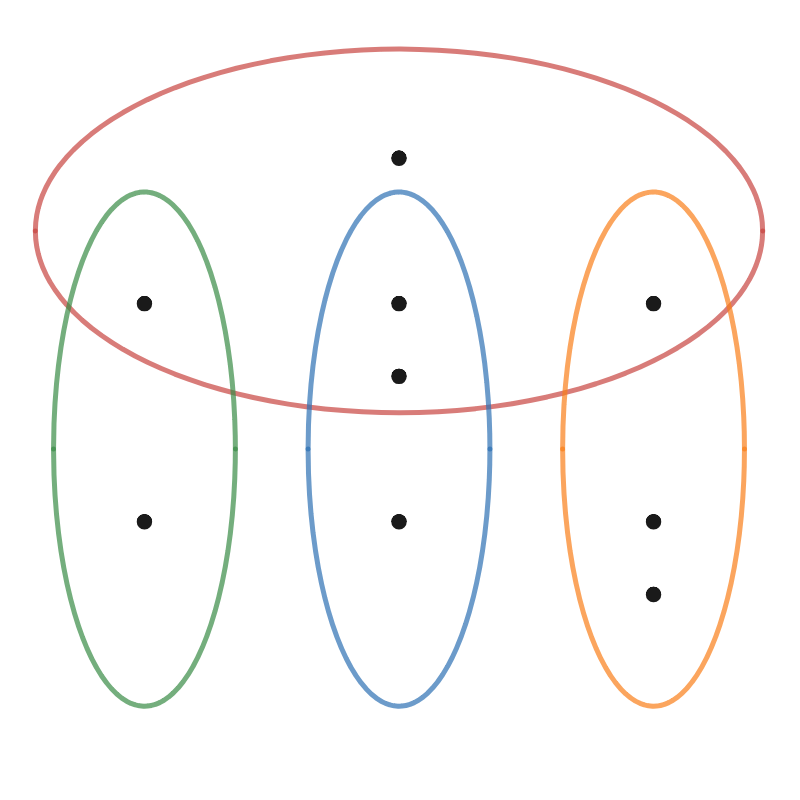
\includegraphics[width=0.6\textwidth]{comb.png}
    \end{subfigure}
    \caption{Comb Inequalities}
\end{figure}

La disuguaglianza afferma che:

\[
    x(E(H)) + \sum_{j=1}^t x(E(T_j)) \leq \abs{H} + \sum_{j=1}^t \abs{T_j} - \frac{3t+1}{2}
\]

Dove \(x(E(S)) = \sum_{e \in E(S)} x_e\) è l'insieme dei lati in un ciclo hamiltoniano i cui vertici appartengono entrambi all'insieme di vertici \(S\subseteq N\). È possibile ricavare tale relazione a partire dai vincoli di grado:
\[
    2x(E(S)) + x(\delta(S)) = 2\abs{S}
\]
Dove \(x(\delta(S)) = \sum_{e \in \delta(S)} x_e\) è l'insieme di lati in un ciclo hamiltoniano che hanno un estremo in \(S\) ed uno in \(N\bs S\).

Riscriviamo la relazione in funzione di \(x\) ed otteniamo:

\[
    x(E(S)) = \abs{S} - \frac{x(\delta(S))}{2}
\]
Sommiamo tale relazione sugli insiemi \(H, T_1, T_2, \ldots, T_t\) ed otteniamo:

\[
    x(E(H)) + \sum_{j=1}^t x(E(T_j)) = \abs{H} + \sum_{j=1}^t \abs{T_j} - \frac{1}{2}\rnd{x(\delta(H))+\sum_{j=1}^t x(\delta(T_j))}
\]

La disuguaglianza a pettine risulta vera se ricaviamo che:

\[
    x(\delta(H)) + \sum_{j=1}^t x(\delta(T_j)) \geq 3t+1
\]

Per farlo procediamo indicando con \(x(\delta_j(H))\) l'insieme dei lati di un ciclo hamiltoniano con un estremo in \(H \cap T_j\) ed uno non in \(H\). Di conseguenza \(x(\delta(H)) \geq \sum_{j=1}^t x(\delta_j(H))\) (il primo termine risulta maggiore perchp vi considero anche i lati di un ciclo hamiltoniano incidenti a vertici in \(H\) ma non nell'intersezione).

Per costruzione del ciclo che può toccare i vertici in \(H\cap T_j\) e \(T_j\bs H\) risulta che:

\[
    x(\delta_j(H)) + x(\delta(T_j)) \geq 3
\]

Unendo le ultime due disuguaglianze si ottiene:

\[
    x(\delta(H)) + \sum_{j=1}^t x(\delta(T_j)) \geq \sum_{j=1}^t x(\delta_j(T)) + \sum_{j=1}^t x(\delta(T_j)) \geq 3t
\]

È noto dalla prima relazione di uguaglianza che \(x(\delta(S))\) sia un valore pari \(\forall S\), mentre \(t\) è per costruzione dispari. Risulta sufficiente aggiungere 1 alla destra della disequazione per ricavare la relazione cercata:

\[
    x(\delta(H)) + \sum_{j=1}^t x(\delta(T_j)) \geq 3t + 1
\]

\end{document}